\documentclass{beamer}

\usepackage{graphicx}
\usepackage{textpos}
\usepackage{dijkstra}
\usepackage{tikz}
\usepackage{verbatim}
\usetikzlibrary{arrows,shapes}

\usetheme{Madrid}
\useoutertheme{miniframes} % Alternatively: miniframes, infolines, split



% Setup the university's color pallette
\definecolor{UIUCorange}{RGB}{19, 41, 75} % UBC Blue (primary)
\definecolor{UIUCblue}{RGB}{232, 74, 39} % UBC Grey (secondary)


\setbeamercolor{palette primary}{bg=UIUCorange,fg=white}
\setbeamercolor{palette secondary}{bg=UIUCblue,fg=white}
\setbeamercolor{palette tertiary}{bg=UIUCblue,fg=white}
\setbeamercolor{palette quaternary}{bg=UIUCblue,fg=white}
\setbeamercolor{structure}{fg=UIUCorange} % itemize, enumerate, etc
\setbeamercolor{section in toc}{fg=UIUCblue} % TOC sections

\setbeamercolor{subsection in head/foot}{bg=UIUCorange,fg=UIUCblue}
\setbeamercolor{subsection in head/foot}{bg=UIUCorange,fg=UIUCblue}

\usepackage[utf8]{inputenc}


%Information to be included in the title page:
\title{\textbf{Dijkstra's Shortest Path\\ and\\ Prim's Minimum Spanning Tree}}
\author{\textbf{Author}}
\institute[\textbf{UIUC}]{\textbf{University of Illinois Urbana-Champaign}}
\date{\textbf{Date}}

\setbeamertemplate{title page}[default][colsep=-4bp,rounded=true]
\addtobeamertemplate{title page}{\vspace{3\baselineskip}}{}
\addtobeamertemplate{title page}{
  \begin{textblock*}{\paperwidth}(-1.0em, -1.2em)
    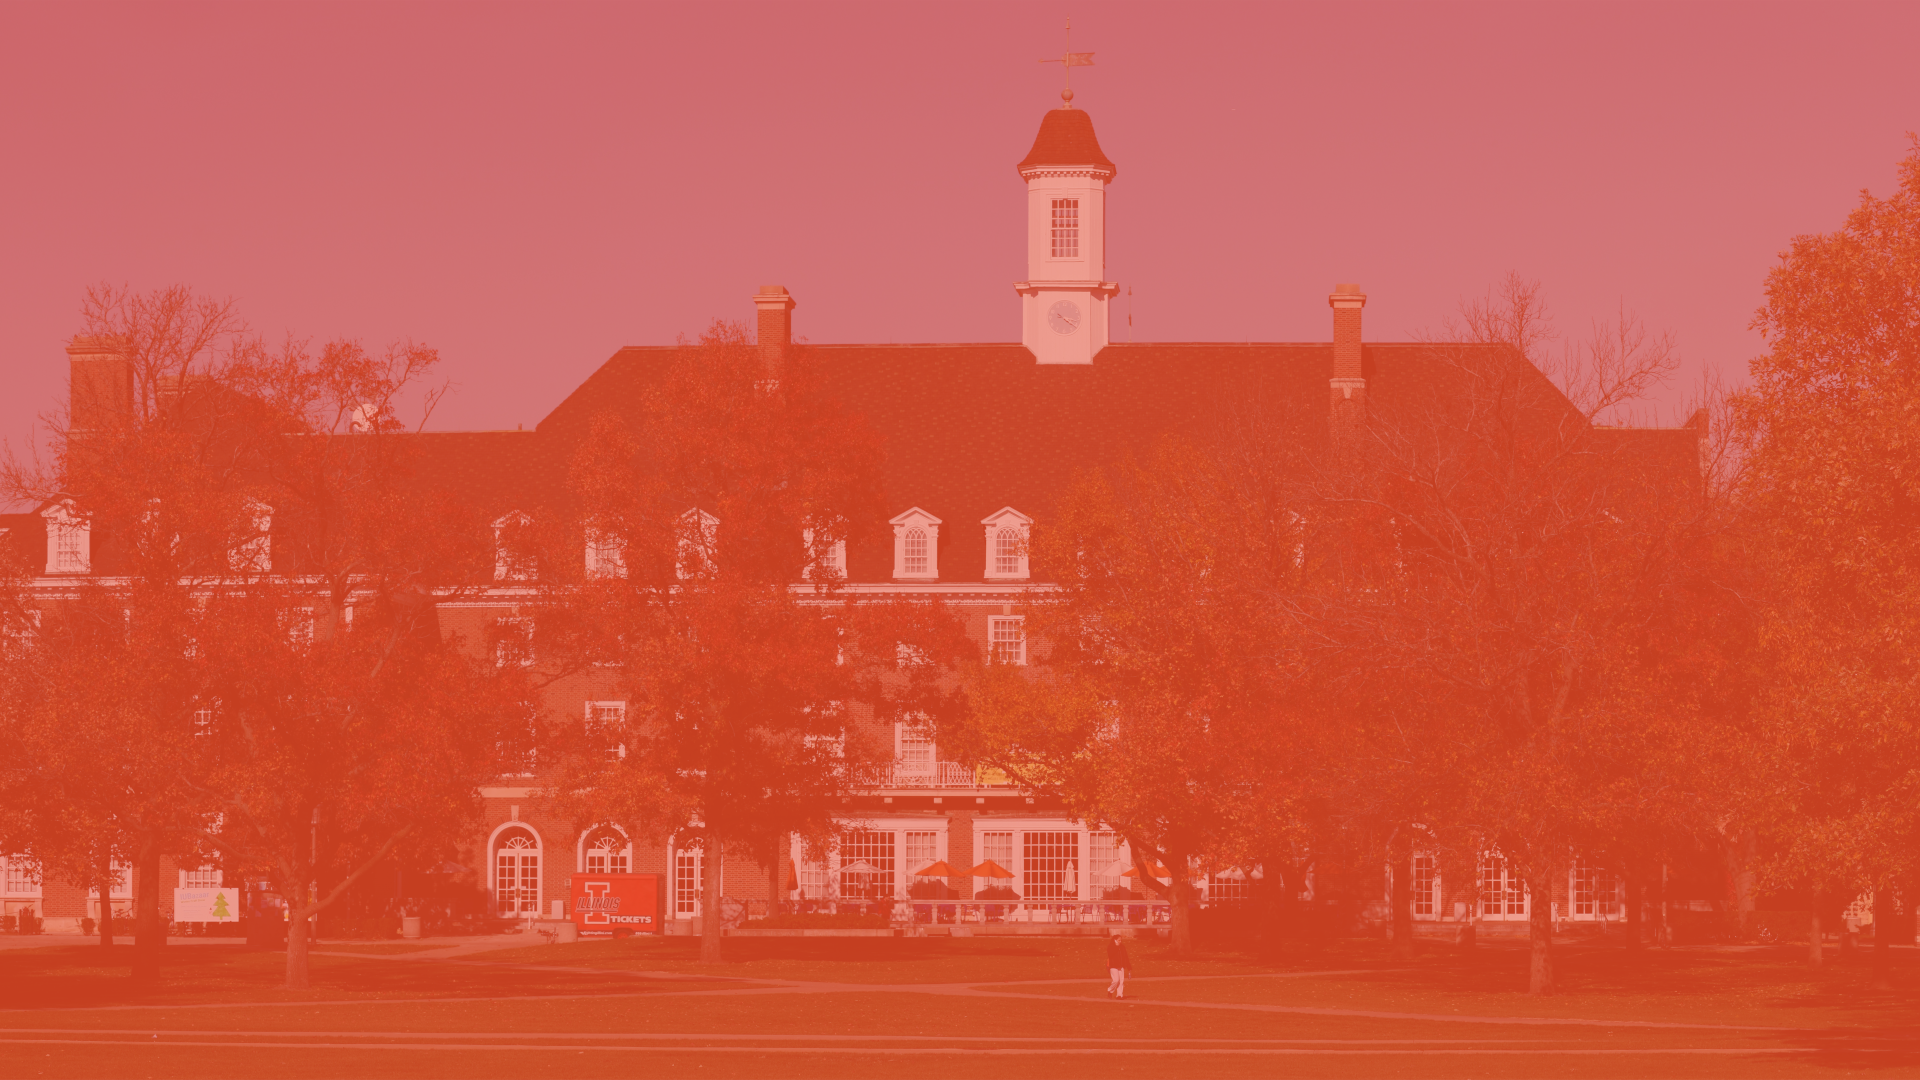
\includegraphics[width=\paperwidth, height=\paperheight]{imgs/uiuc.png}
  \end{textblock*} 
}{}

\begin{document}

\pgfdeclarelayer{background}
\pgfsetlayers{background,main}

\tikzstyle{vertex}=[circle,fill=black!25,minimum size=20pt,inner sep=0pt]
\tikzstyle{selected vertex} = [vertex, fill=orange!24]
\tikzstyle{edge} = [draw,thick,-]
\tikzstyle{weight} = [font=\small]
\tikzstyle{selected edge} = [draw,line width=5pt,-,blue!50]
\tikzstyle{ignored edge} = [draw,line width=5pt,-,black!20]


\frame{\titlepage}

\section{Prim's Algorithm - Walkthrough}
\begin{frame}
    \centering
    \begin{tikzpicture}[scale=1.8, auto,swap]
        % Draw a 7,11 network
        % First we draw the vertices
        \foreach \pos/\name in {{(0,1)/a}, {(2,1)/b}, {(4,1)/c},
                                {(0,0)/d}, {(3,0)/e}, {(2,-1)/f}, {(4,-1)/g}}
            \node[vertex] (\name) at \pos {$\name$};
        % Connect vertices with edges and draw weights
        \foreach \source/ \dest /\weight in {b/a/7, c/b/8,d/a/5,d/b/9,
                                             e/b/7, e/c/5,e/d/15,
                                             f/d/6,f/e/8,
                                             g/e/9,g/f/11}
            \path[edge] (\source) -- node[weight] {$\weight$} (\dest);
        % Start animating the vertex and edge selection. 
        \foreach \vertex / \fr in {d/1,a/2,f/3,b/4,e/5,c/6,g/7}
            \path<\fr-> node[selected vertex] at (\vertex) {$\vertex$};
        % For convenience we use a background layer to highlight edges
        % This way we don't have to worry about the highlighting covering
        % weight labels. 
        \begin{pgfonlayer}{background}
            \pause
            \foreach \source / \dest in {d/a,d/f,a/b,b/e,e/c,e/g}
                \path<+->[selected edge] (\source.center) -- (\dest.center);
            \foreach \source / \dest / \fr in {d/b/4,d/e/5,e/f/5,b/c/6,f/g/7}
                \path<\fr->[ignored edge] (\source.center) -- (\dest.center);
        \end{pgfonlayer}
    \end{tikzpicture}
\end{frame}


\section{Dijkstra's Walkthrough}
\begin{frame}
  \frametitle{Dijkstra's Table}
    \readgraph*{
        A [B=7, D=5],
        B [D=9, E=7, C=8],
        C [E=5],
        D [E=15, F=6],
        E [F=8, G=9],
        F [F=8, G=11],
        G [F=11]
    }
    \centering
    \dijkstra{A}{G}\par
    \vspace{0.1cm}
    Distance: A-G= \dijkdist\par\\
    Path: \dijkpath\\
\end{frame}


\end{document}
